% Remplacement local des trois encadrés d'attente du chapitre Data/IA.
% Ce fichier est chargé dans un groupe LaTeX dédié depuis main.tex : la
% redéfinition de \fbox ne s'applique donc pas au reste du dossier.
\newcounter{dataiafigureplaceholder}
\setcounter{dataiafigureplaceholder}{0}
\let\dataiaoriginalfbox\fbox

\renewcommand{\fbox}[1]{%
  \stepcounter{dataiafigureplaceholder}%
  \ifcase\value{dataiafigureplaceholder}%
    \dataiaoriginalfbox{#1}%
  \or
    % Analyse exploratoire : trois graphiques issus du notebook.
    \begin{minipage}{0.98\textwidth}
      \centering
      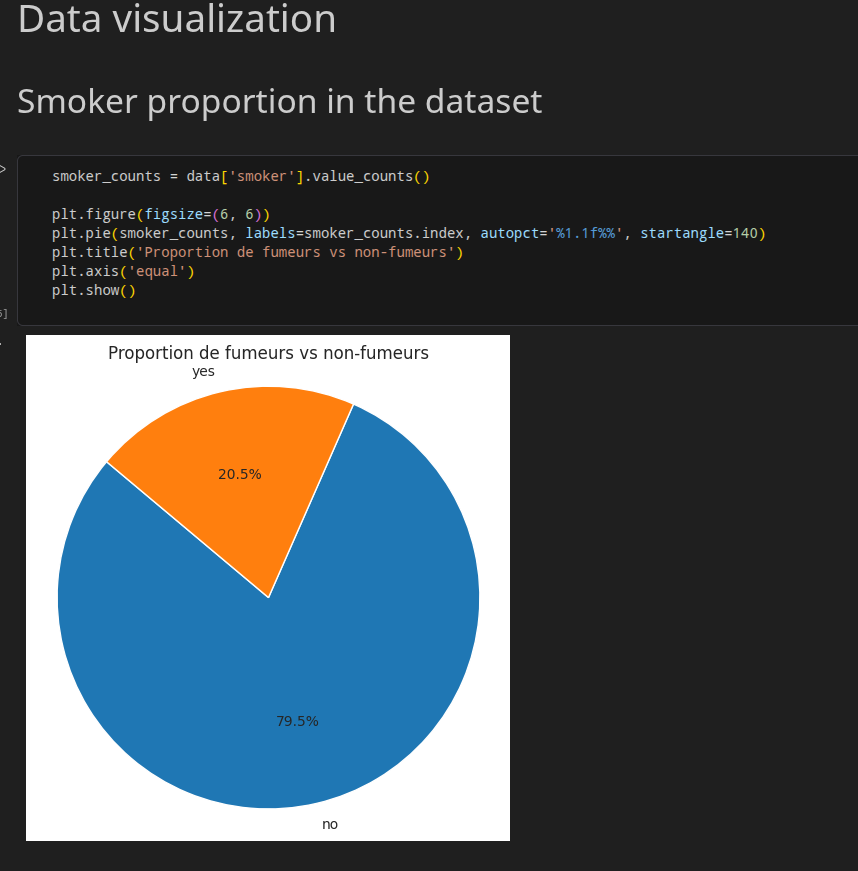
\includegraphics[width=0.48\textwidth,height=0.25\textheight,keepaspectratio]{figures/ia/fumeur_non_fumeur.png}\hfill
      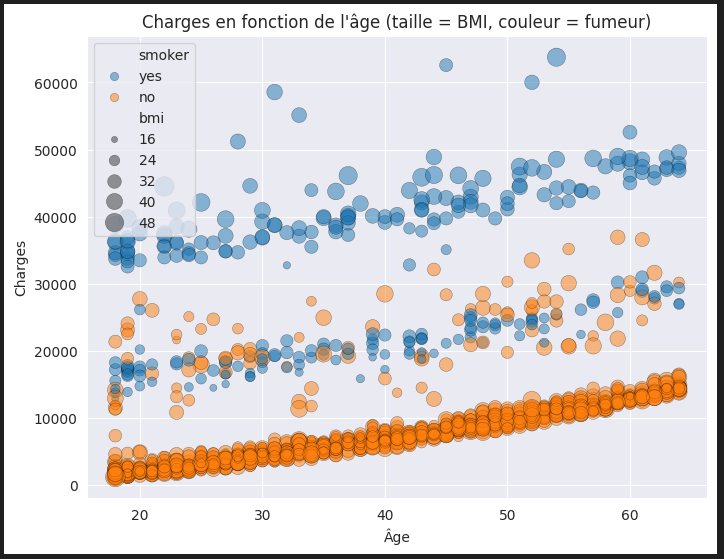
\includegraphics[width=0.48\textwidth,height=0.25\textheight,keepaspectratio]{figures/ia/charge_en_function_de_l_age.png}\\[0.4cm]
      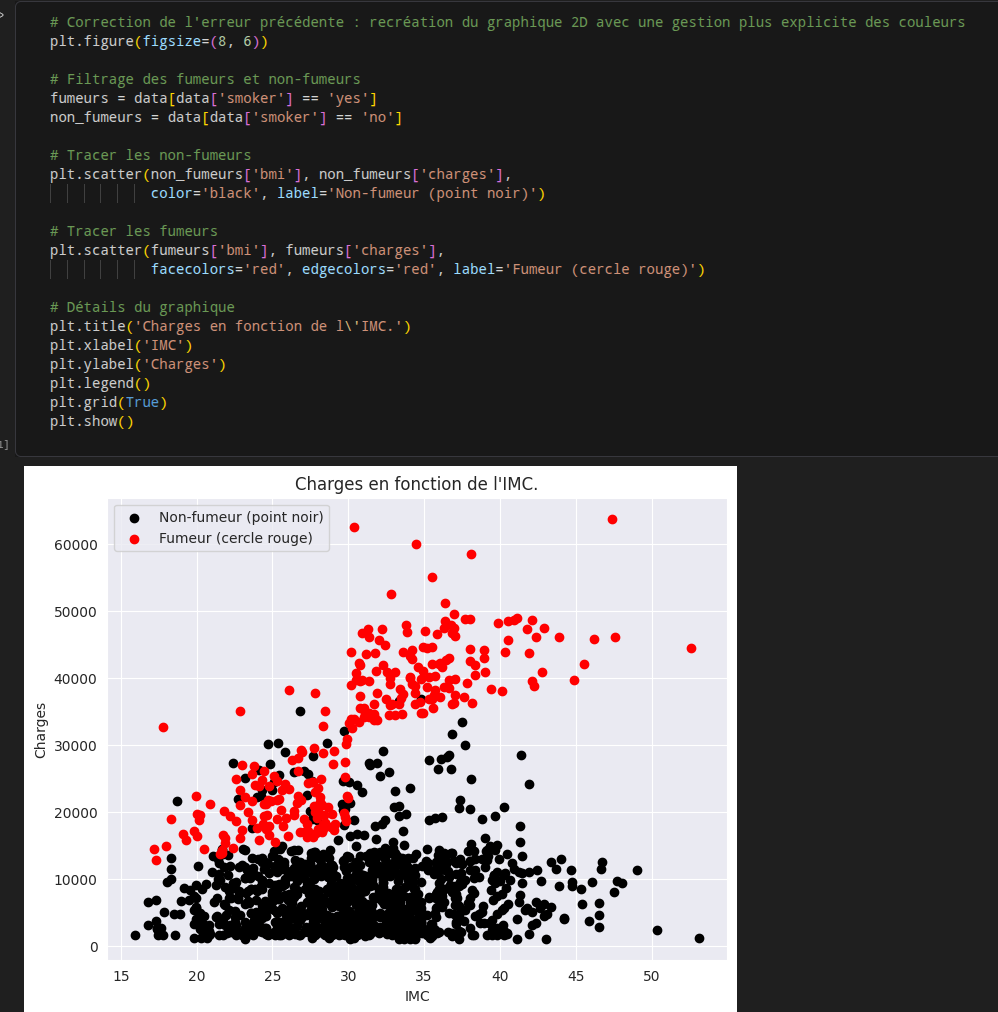
\includegraphics[width=0.62\textwidth,height=0.27\textheight,keepaspectratio]{figures/ia/charge_imc.png}
    \end{minipage}%
  \or
    % Architecture effectivement développée.
    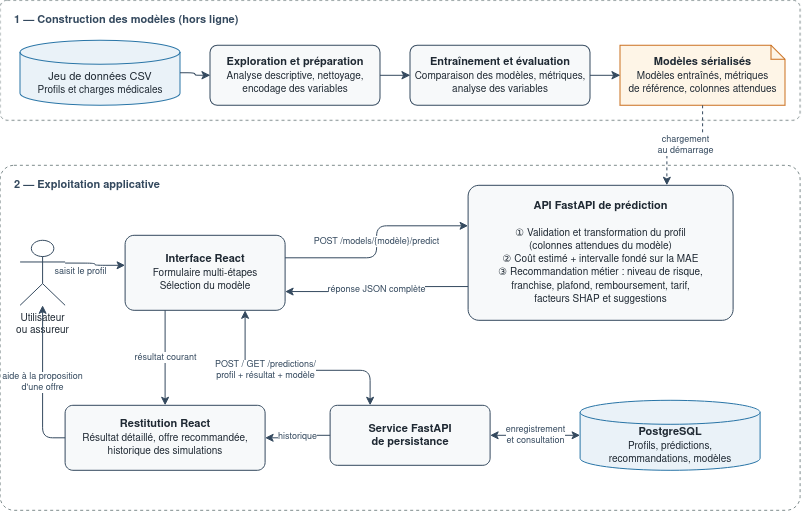
\includegraphics[width=0.94\textwidth,height=0.63\textheight,keepaspectratio]{figures/ia/architecture_actuelle.png}%
  \or
    % Architecture cible volontairement simplifiée dans le corps du dossier.
    \begin{minipage}{0.98\textwidth}
      \centering
      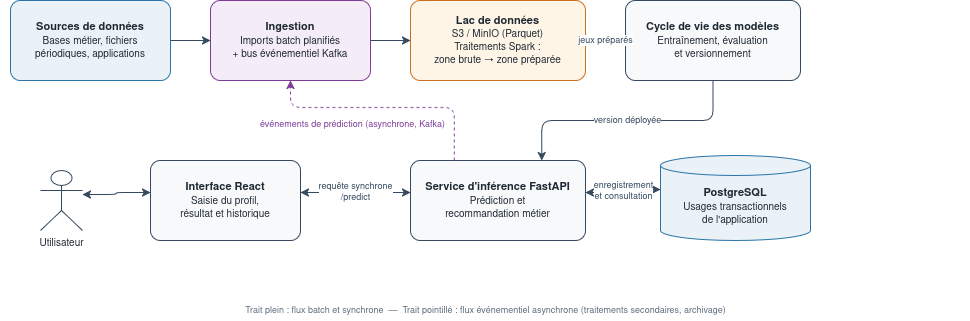
\includegraphics[width=0.94\textwidth,height=0.58\textheight,keepaspectratio]{figures/ia/nouvelle_architecture_simplifie.png}\\[0.25cm]
      \small\emph{Cette représentation est volontairement simplifiée afin de conserver une lecture claire dans le chapitre. La version complète de l'architecture cible est présentée en annexe~\ref{ann:data-ia-architecture-complete}.}
    \end{minipage}%
  \else
    \dataiaoriginalfbox{#1}%
  \fi
}
